\chapter{Testing and Application} \label{ch:04}

This chapter contains an overview of the tests performed during the development of \stops\ which includes the verification of the modified wavelength solutions (\autoref{sec:test_stops}), as well as the application of \stops\ on observations of both spectrophotometric standards and science targets (\autoref{sec:app_stops}).

% MARK: Test STOPS
\section[Testing \textsc{stops}]{Testing \stops} \label{sec:test_stops}

% No \polsalt\ tests or tests on pre-reduced \gls{FITS} files. (Trusted accurate)

% % Why the pipeline is better
% The rigorous error handling in \stops\ ensures that the user is informed of any issues that arise during the reduction process. This is particularly important as \stops\ was developed to enable a faster reduction process compared to that of pure \iraf\ or \polsalt.

A fundamental requirement during the development of \stops\ was ensuring that the software was compatible with both the \polsalt\ and \iraf\ file structures and that the `reduction-specific' methods, namely the \stops\ \texttt{split} and \texttt{join} methods, provided correct and consistent results.
As development is an iterative process, \stops\ was continually checked to ensure compatibility such that the varying \stops\ method inputs were correctly parsed, and that their outputs were parsable by the relevant \iraf\ tasks or \polsalt\ methods.

To this end, observations which were verified to have been accurately reduced were duplicated for testing the `reduction-specific' methods, allowing for continual checks of the \stops\ pipeline to be made during the development process.
The testing of the `reduction-specific' methods are discussed in \autoref{subsec:test_split} and \autoref{subsec:test_join}, respectively.

% No \iraf\ tests or tests on \iraf\ \gls{FITS} files. (Trusted accurate)
The secondary requirement during the development of \stops\ was to provide a means to check the wavelength solutions.
This was achieved through the `check-specific' methods, namely the \stops\ \texttt{correlate} and \texttt{skylines} methods, which were designed to validate the \iraf\ wavelength solutions, specifically after re-insertion of the wavelength solutions back into the \polsalt\ \gls{FITS} file format.
The file format distinction is necessary as \iraf\ provides immediate confirmation of the wavelength solutions during calibration through interactive \gls{RMS} plots (see e.g. \autoref{fig:iraf_id_plot}, \ref{fig:iraf_fc_plot}), as well as the transformation of the spectra through the \texttt{transform} \iraf\ task, while \polsalt\ only provides confirmation of the \gls{RMS} for the interactive line identification during \texttt{wavelength calibration}.

% The \texttt{correlate} method provides a means to confirm the relative offsets in the wavelength solutions across polarization beams (as well as across the related \gls{CCD}['s]), and as such was tested by correlating two synthetic spectra with a feature in each \gls{CCD} offset by a varying amount.
% The \texttt{skylines} method provides a means to confirm the accuracy of the wavelength solution by attempting to retrieve and compare the skylines from a spectrum, which are not used during wavelength calibration and thus correlate well to the fit of the wavelength solution, to skylines as measured by \gls{SALT}, and as such was tested using a synthetic spectrum with artificial skylines added which were offset by varying amounts.
The `check-specific' methods were tested using synthetic spectra, which contained features with known and varying offsets introduced.
The features refer to emission lines in the \texttt{correlate} related tests and absorption skylines in the \texttt{skylines} related tests.
The testing of the `check-specific' methods are discussed in \autoref{subsec:test_corr} and \autoref{subsec:test_sky}, respectively.

% MARK: STOPS split tests
\subsection{Testing the \texttt{split} Method} \label{subsec:test_split}

The \stops\ \texttt{split} method accepts any \polsalt\ pre-reduced (`mxgbp'- prefixed) \gls{FITS} files as input and outputs \iraf\ compatible (`[arc|beam][o|e]'- prefixed) \gls{FITS} file structures.
As no `split' \gls{FITS} files are created during pure \polsalt\ reductions, the \stops\ \texttt{split} method was tested by comparing the pre-reduced \polsalt\ files to the \texttt{split} method's output files, ensuring the correct structure and data integrity of the files to be handed off to \iraf.

% \newcommand\mc[1]{\multicolumn{1}{c|}{#1}} % handy shortcut macro

\begin{table}[t]

    \centering

    \caption{A comparison of the contents of a \polsalt\ pre-reduced \gls{FITS} file to the \stops\ \texttt{split} $O$- and $E$-beam \gls{FITS} files. Table created using the `\texttt{Astropy}' \texttt{fitsinfo} \gls{CLI} tool.}
    \label{table:split_info}

    \begin{tabular}{lcccccc}
        \toprule
        Filename &
        No. &
        Name &
        Type &
        Cards &
        Dimensions &
        Format \\
        \midrule
        \polsalt % mxgbpP201703280054.fits
        & $0$ & \gls{PRIMARY} & PrimaryHDU & $161$   & -                & -       \\
        & $1$ & \gls{SCI}     & ImageHDU   & $19$    & ($3199$, $1028$) & float32 \\
        & $2$ & \gls{VAR}     & ImageHDU   & $8$     & ($3199$, $1028$) & float32 \\
        & $3$ & \gls{BPM}     & ImageHDU   & $8$     & ($3199$, $1028$) & uint8   \\
        \stops\ \texttt{split} `$O$' % beamo0054.fits
        & $0$ & \gls{PRIMARY} & PrimaryHDU & $162$   & ($3199$, $474$)  & float32 \\
        \stops\ \texttt{split} `$E$' % beame0054.fits
        & $0$ & \gls{PRIMARY} & PrimaryHDU & $162$   & ($3199$, $474$)  & float32 \\ \bottomrule
    \end{tabular}

\end{table}


\autoref{table:split_info} shows the contents of a \gls{FITS} file before and after splitting.
The split \gls{FITS} files contain a single \gls{PRIMARY} extension which holds the respective polarization beams' two-dimensional spectrum as well as a slightly modified copy of the \gls{PRIMARY} header from the `pre-split' file. The differences in the header and data are detailed below.

For the split \gls{FITS} files, the header is left mostly untouched, and is only updated to represent the new data type and shape:
the `BITPIX' value is updated, from $8$ to $-32$, and the `NAXIS' value is updated, from $0$ to $2$;
the `NAXIS1' and `NAXIS2' keywords are added, and their values are set to the new split \gls{SCI} data shape;
and the `EXTEND' keyword is removed.%
\footnote{The `EXTEND' keyword indicates that the \gls{FITS} file contains multiple extensions while the `NAXIS1' and `NAXIS2' keywords indicate the shape and size of the data stored in the relevant extension.}
This accounts for the discrepancy in the `Cards' between the \polsalt\ and \stops\ file header entries in \autoref{table:split_info}.

% \begin{figure}
%     \centering
%     \begin{subfigure}[b]{\textwidth}
%         \centering
%         
\includegraphics[width=\textwidth]{4_diff_O.pdf}
%         \caption{The difference in the \gls{SCI} extensions, for the `O' polarization beam.}
%         \label{subfig:diff_split_O}
%     \end{subfigure}
%     \hfill
%     \begin{subfigure}[b]{\textwidth}
%         \centering
%         
\includegraphics[width=\textwidth]{4_diff_E.pdf}
%         \caption{The difference in the \gls{SCI} extensions, for the `E' polarization beam.}
%         \label{subfig:diff_split_E}
%     \end{subfigure}
%     \caption{The difference between the \polsalt\ pre-reduced (`mxgbp'- prefixed) \gls{FITS} files and the \stops\ `split' (`[arc|beam][o|e]'- prefixed) files. Figures created using both the \polsalt\ \texttt{Raw image reduction} and \stops\ \texttt{split} method outputs.}
%     \label{fig:split_diff}
% \end{figure}

% \autoref{fig:split_diff} shows that the \polsalt\ \gls{SCI} data is unmodified when copying the data to the \stops\ \gls{FITS} file, although each file only includes half of the data, for the relevant $O$- or $E$-polarization beam, \autoref{subfig:diff_split_O} and \autoref{subfig:diff_split_E}, respectively.
% The split data is also cropped at the top- and bottom-most rows of the \polsalt\ data, with the cropping defaulting to $40$~pixels (see \autoref{subsec:stops_split}).
% This accounts for the discrepancy in the `Dimensions' between the \polsalt\ and \stops\ files in \autoref{table:split_info}.

After splitting it was confirmed that the split data was identical to the \polsalt\ `pre-split' file by taking the difference between them, which showed a constant difference of zero.
Each split \gls{FITS} file, however, only includes half of the `pre-split' data, for the relevant $O$- or $E$-polarization beam, with the data also being cropped at the top- and bottom-most rows of the \polsalt\ data, with the cropping defaulting to $40$~pixels (see \autoref{subsec:stops_split}). This accounts for the discrepancy in the `Dimensions' between the \polsalt\ and \stops\ files in \autoref{table:split_info}.

This output file structure was chosen for \iraf\ compatibility, and was tested over multiple grating and articulation angles, as well as with various data sets to ensure that the \texttt{split} method was robust and reliable.

% MARK: STOPS join tests
\subsection{Testing the \texttt{join} Method} \label{subsec:test_join}

The \texttt{join} method requires both an \iraf\ database with wavelength solutions%
\footnote{A custom wavelength solution may also be used.}
for both polarimetric beams, and the \polsalt\ pre-reduced files as input,  and outputs \polsalt\ \texttt{spectra extraction} compatible (`wmxgbp'- prefixed) \gls{FITS} files.
Ensuring that the output format was correct was paramount as the \polsalt\ \texttt{spectra extraction} method is unable to process the files otherwise, thus halting the reduction process.
Thankfully, the \texttt{join} method output could be directly compared to the \polsalt\ \texttt{wavelength calibration} method output files, ensuring that any changes introduced by the \stops\ pipeline are well characterized.

\begin{table}[t]

    \centering

    \caption{A comparison of the \polsalt\ wavelength calibrated \gls{FITS} file to the (\iraf\ wavelength calibrated) \stops\ \texttt{join} \gls{FITS} file. Table created using the \texttt{Astropy} \texttt{fitsinfo} \gls{CLI} tool.}
    \label{table:join_info}

    \begin{tabular}{lcccccc}
        \toprule
        Filename &
        Ext. No. &
        Name &
        Type &
        Cards &
        Dimensions &
        Format \\
        \midrule
        \polsalt % wmxgbpP201703280054.fits
        & $0$ & \gls{PRIMARY} & Primary\gls{HDU} & $161$ & -             & -       \\
        & $1$ & \gls{SCI} & Image\gls{HDU} & $21$ & ($3199$, $514$, $2$) & float32 \\
        & $2$ & \gls{VAR} & Image\gls{HDU} & $10$ & ($3199$, $514$, $2$) & float32 \\
        & $3$ & \gls{BPM} & Image\gls{HDU} & $10$ & ($3199$, $514$, $2$) & uint8   \\
        & $4$ & \gls{WAV} & Image\gls{HDU} & $21$ & ($3199$, $514$, $2$) & float32 \\
        \stops\ \texttt{join} % wmxgbpP201703280054.fits
        & $0$ & \gls{PRIMARY} & Primary\gls{HDU} & $161$ & -             & -       \\
        & $1$ & \gls{SCI} & Image\gls{HDU} & $21$ & ($3199$, $474$, $2$) & float32 \\
        & $2$ & \gls{VAR} & Image\gls{HDU} & $10$ & ($3199$, $474$, $2$) & float32 \\
        & $3$ & \gls{BPM} & Image\gls{HDU} & $10$ & ($3199$, $474$, $2$) & uint8   \\
        & $4$ & \gls{WAV} & Image\gls{HDU} & $21$ & ($3199$, $474$, $2$) & float32 \\
        \bottomrule
    \end{tabular}

\end{table}


\autoref{table:join_info} shows the \gls{FITS} file information for both the \polsalt\ and \stops\ wavelength calibrated files.
Other than the `Dimensions' of each `ImageHDU' extension, the \gls{FITS} files have identical structures.%
\footnote{The `Dimensions' differ due to the aforementioned cropping of the top- and bottom-most rows of the pre-reduced \gls{FITS} files data.}

Although the `Cards' count is the same, minor differences across the headers are present.
The `HISTORY' keyword, which would have contained the \polsalt\ `CRCLEAN' parameters, and which default to `upper= 4.0, lower= 1.5, sigmaveto= 2.0', is instead modified to contain the implemented \gls{CRR} parameters.%
\footnote{The \polsalt\ pipeline performs \gls{CRR} using a $10\sigma$ spike to cull cosmic rays. See the \protect\href{https://github.com/saltastro/polsalt/blob/master/polsalt/specpolwavmap.py\#L132}{source code} of \polsalt\ for more information.}
% Although \stops\ performs \gls{CRR} (see \autoref{subsec:stops_join}), the parameters are not stored in the header as \polsalt\ and \stops\ implement different methods for \gls{CRR}.  % Deprecated as the parameters *are* now stored in the header.

\begin{figure}
    \centering
    \begin{subfigure}[b]{\textwidth}
        \centering
        
\includegraphics[width=\textwidth]{4_diff_SCI.pdf}
        \caption{The difference in the \gls{SCI} extensions.}
        \label{subfig:join_SCI}
    \end{subfigure}
    \hfill
    \begin{subfigure}[b]{\textwidth}
        \centering
        
\includegraphics[width=\textwidth]{4_diff_VAR.pdf}
        \caption{The difference in the \gls{VAR} extensions.}
        \label{subfig:join_VAR}
    \end{subfigure}
    \hfill
    \begin{subfigure}[b]{\textwidth}
        \centering
        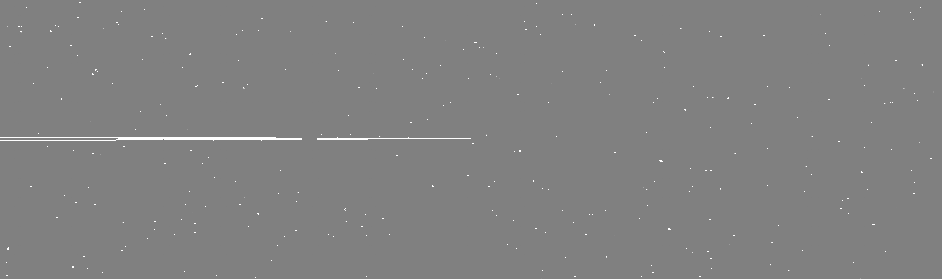
\includegraphics[width=\textwidth]{4_diff_BPM.pdf}
        \caption{The difference in the \gls{BPM} extensions.}
        \label{subfig:join_BPM}
    \end{subfigure}
    \hfill
    \begin{subfigure}[b]{\textwidth}
        \centering
        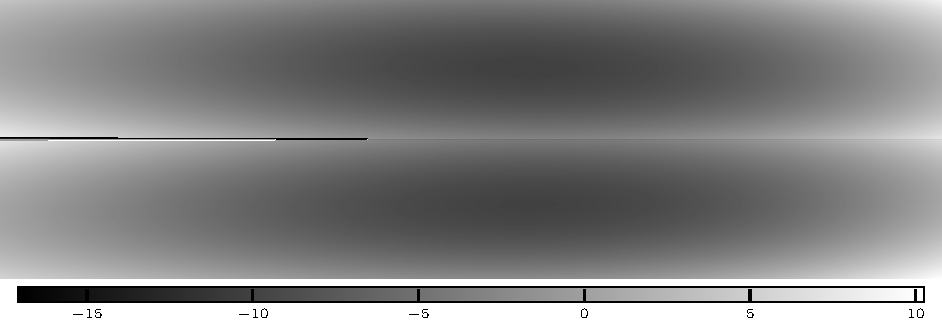
\includegraphics[width=\textwidth]{4_diff_WAV.pdf}
        \caption{The difference in the \gls{WAV} extensions.}
        \label{subfig:join_WAV}
    \end{subfigure}
    \caption{The difference of the \gls{FITS} file extensions between the \polsalt\ and \stops\ (`wmxgbp'- prefixed) wavelength calibrated files. Figures created using both the \polsalt\ and \stops versions of the \polsalt\ \texttt{spectral extraction} input.}
    \label{fig:join_in_out_diff}
\end{figure}

Other minor differences may arise, such as the date-times stored in the `SAL-TLM' and `SMOSAIC' keywords, as they contain the date-times relating to the completion of the \polsalt\ pre-reductions.
This accounts for the differences in the `Cards' between the \polsalt\ and \stops\ file header entries in \autoref{table:join_info}.

\autoref{fig:join_in_out_diff} shows the differences in the data between the \polsalt\ and \stops\ wavelength calibrated files.
It can be seen that the \gls{VAR} extensions (\autoref{subfig:join_VAR}) are identical.
The difference in the \gls{SCI} extensions (\autoref{subfig:join_SCI}) is due to the \gls{CRR} applied by \stops\, which rejects cosmic rays from the \gls{SCI} extension instead of masking the \gls{BPM} extension (\autoref{subfig:join_BPM}) which is the method implemented by \polsalt.
The valid wavelength calibrated region is used as a mask and applied to the \gls{BPM} and \gls{WAV} extensions (\autoref{subfig:join_WAV}).
Slight differences arise near the centre of the frames, specifically \autoref{subfig:join_BPM} and \ref{subfig:join_WAV}, since the correction for the wollaston tilt, as implemented by \polsalt, is re-implemented in Python~$3$ by \stops\ and as such may be affected by rounding differences.
The differences are fortunately minor and are at the edges of the two polarimetric spectral regions
The \gls{WAV} extensions contain the differing wavelength solutions and as such naturally differ.
This accounts for the differences in the data between the \polsalt\ and \stops\ files.

Finally, the \stops\ \texttt{join} method was tested to ensure compatibility and correctness of the output data in comparison to \polsalt.
This involved testing the \texttt{join} method with various data sets, with differing observation configurations, to ensure that the output files were accurate and consistent.

% MARK: WAV Corr. Checks
\subsection{Cross Correlation Checks} \label{subsec:test_corr}

% O/E correlation checks to verify the consistency of the wavelength solutions.
The \texttt{correlate} method returns plots validating the wavelength solutions and so only has to accept the files output from the \polsalt\ \texttt{spectra extraction}  method (`ecwmxgbp'- prefixed files).

\begin{figure}
    \centering
    \begin{subfigure}[b]{\textwidth}
        \centering
        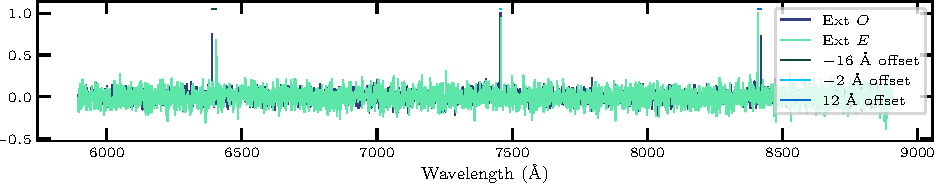
\includegraphics[width=\textwidth]{4_corr_spec.pdf}
        \caption{Synthetic $O$- and $E$-beam spectra.}
        \label{subfig:corr_test_spec}
    \end{subfigure}
    \hfill
    \begin{subfigure}[b]{\textwidth}
        \centering
        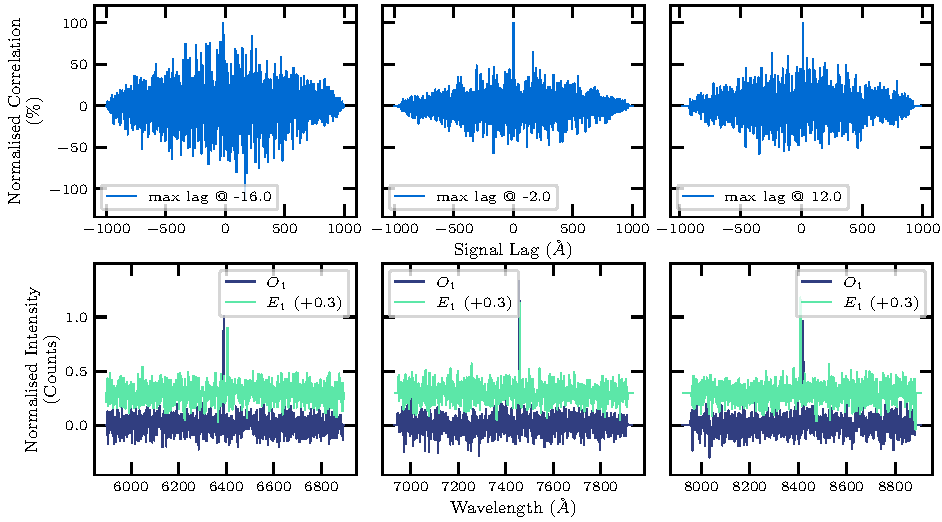
\includegraphics[width=\textwidth]{4_corr_test.pdf}
        \caption{The \stops\ \texttt{correlate} result for the spectra displayed in \subref{subfig:corr_test_spec}.}
        \label{subfig:corr_test_corr}
    \end{subfigure}
    \caption{Reacquisition of offsets introduced to the $O$- and $E$-beam spectral features (\subref{subfig:corr_test_spec}) by cross-correlation (\subref{subfig:corr_test_corr}, bottom row).}
    \label{fig:corr_test}
\end{figure}

The \stops\ \texttt{correlate} method was tested by cross correlating synthetic $O$- and $E$-beam spectra with known offsets, with the aim of reacquiring said offsets, as shown in \autoref{fig:corr_test}.
The spectra were generated with a feature in each \gls{CCD} region, randomly offset in both the wavelength and intensity axes, \autoref{subfig:corr_test_spec}.
The features were purposefully chosen to be of low \gls{SNR}['s] and \gls{FWHM} to test the robustness of the \texttt{correlate} method.
Non-synthetic spectra will include more features, with higher \gls{SNR}['s] and \gls{FWHM}, and as such will be more robust to the \texttt{correlate} method.

Through cross correlation, \autoref{subfig:corr_test_corr}, the introduced offsets, or `max lag', were reacquired.
For spectral regions with few features or features with a low \gls{SNR} (such as the left most \gls{CCD} region of \autoref{subfig:corr_test_corr}), correlation may fail to determine the correct offset.
When a returned `max lag' peak is not significant when compared to the noise in the correlation plots, the \gls{SNR} of the features may be too low for an accurate calculation of the offset.

% MARK: WAV Sky. Checks
\subsection{Sky Line Checks} \label{subsec:test_sky}

% Full frame wavelength solution checks to ensure comprehensive calibration.
% Verifying the accuracy of the cross-correlation function against known standards.
The \texttt{skylines} method returns plots validating the wavelength solutions and so has to accept as input the files output from the \stops\ \texttt{join} method.

\begin{figure}[t]
    \centering
    \begin{subfigure}[b]{1.0 \textwidth}
        \centering
        \includegraphics[width = 1.0\textwidth]{4_sky_test.pdf}
        \caption{A generated two-dimensional spectrum consisting of noise, skyline emission features, and the characteristic \gls{RSS} chip gaps.}
        \label{subfig:sky_test_spec}
    \end{subfigure}
    \hfill
    \begin{subfigure}[b]{1.0 \textwidth}
        \centering
        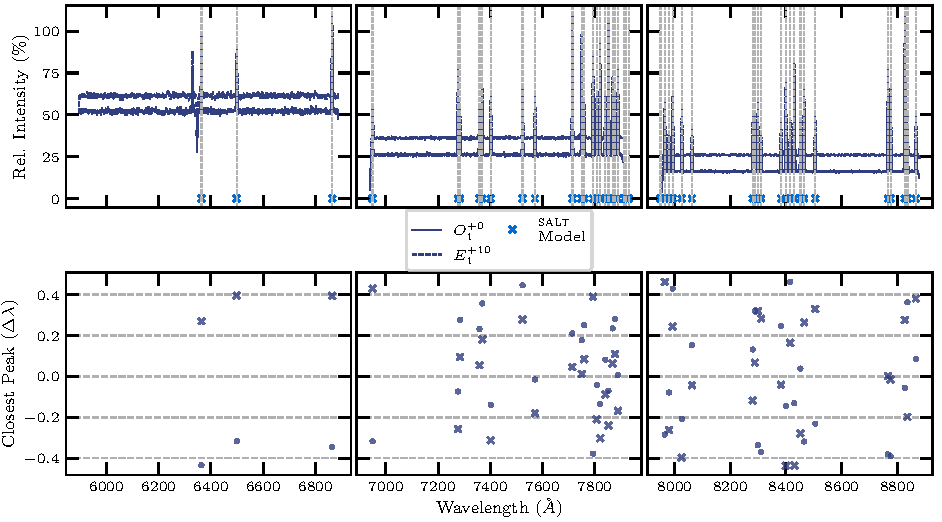
\includegraphics[width = 1.0\textwidth]{4_sky_test_pure.pdf}
        \caption{The \stops\ \texttt{skylines} output for the synthetic spectrum displayed in \subref{subfig:sky_test_spec}.}
        \label{subfig:sky_test_pure}
    \end{subfigure}
    \caption{The \stops\ \texttt{skylines} method output \subref{subfig:sky_test_pure} for a synthetic two-dimensional spectrum \subref{subfig:sky_test_spec}. Figures generated using Python \subref{subfig:sky_test_spec} and the \stops\ \texttt{skylines} method \subref{subfig:sky_test_pure}.}
    \label{fig:sky_test}
\end{figure}

In order to validate the \stops\ \texttt{skylines} method, a synthetic two-dimension spectrum was created that contained sky lines. This is shown in \autoref{subfig:sky_test_spec}, and consists of an average continuum ($10$~`counts') with added noise (normal-sampled, $\sigma = 4.5$), skyline emission features (provided by \gls{SALT}, see \autoref{subsec:stops_skyline}), and the characteristic \gls{RSS} chip gaps.
% The two-dimensional spectrum was used to test the \stops\ \texttt{skylines} method.
\autoref{subfig:sky_test_pure} shows the result, which successfully retrieves the skyline emission features for the synthetic spectrum.
Note that the closest peaks ($\Delta \lambda$) are nearly never $0$, since the skylines are only as accurate as the spectral pixel resolution ($\sim~1$~\AA\ in our synthetic spectrum) while those as provided by \gls{SALT} are not similarly limited.
Additionally, the noise in the spectrum may shift a skylines' peak position, further contributing to, albeit small, discrepancies.

\begin{figure}[t]
    \centering
    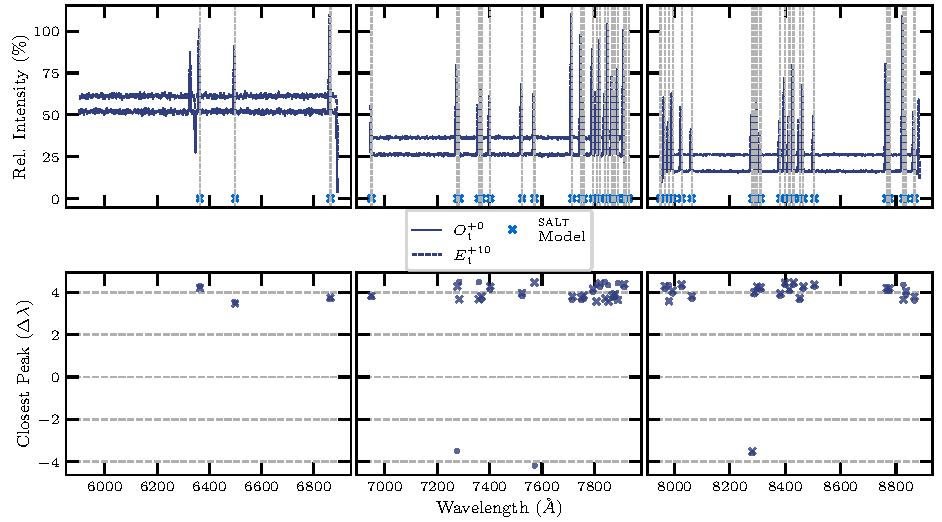
\includegraphics[width = 1.0\textwidth]{4_sky_test_shift.pdf}
    \caption{The \stops\ \texttt{skylines} output for a two-dimensional spectrum, as described in \autoref{subfig:sky_test_pure}, with a constant offset of $4$~\AA\ applied to all skyline emission features. Figure created using the \stops\ \texttt{skylines} method.}
    \label{fig:sky_test_shift}
\end{figure}

\autoref{fig:sky_test_shift} shows the result of the \stops\ \texttt{skylines} method when a constant offset of $4$~\AA\ is applied to all skyline emission features in \autoref{subfig:sky_test_spec}.
In general, the offset is recovered, with the minor variation in the closest peaks once again noticed.
The closest peaks near $\Delta \lambda \sim -4$~\AA\ are the most notable outliers, and are due to misidentifications of skyline features with neighbors closer than $8$~\AA.

% MARK: Application
\section[Application of \textsc{stops}]{Application of \stops} \label{sec:app_stops}
% https://ui.adsabs.harvard.edu/search/fq=%7B!type%3Daqp%20v%3D%24fq_database%7D&fq_database=database%3Aastronomy&p_=0&q=%20author%3A%22Cooper%2C%20J.%22%20spectropolarimetry&sort=date%20desc%2C%20bibcode%20desc

% Sources are blazars
% The \stops\ pipeline has been utilized in the reduction of a number of science targets, specifically focused on blazars.
The \stops\ pipeline has been utilized for the reduction of a number of sources: this includes calibration tests using spectropolarimetric standards; and for scientific observations of transient sources, specifically \gls{GRB}['s] and blazars.
The following sections summarize works in which observations were analysed using, in part, the \stops\ pipeline with \iraf\ wavelength calibrations, or from which the \stops\ pipeline was developed.
The list of sources observed are summarized in \autoref{table:sci_targets}.
In addition to the results discussed here, the \stops\ pipeline has also been extensively used for the analysis of the blazers presented in \citet{Barnard_HEASA2021, Barnard_2024}.

\begin{table}[t]
    \centering
    \begin{tabular}{cccccc}
        \toprule
        Source & \begin{tabular}[c]{@{}c@{}}Observation\\ Date\end{tabular} & Grating & \begin{tabular}[c]{@{}c@{}}Grating\\ Angle (\degree)\end{tabular} & \begin{tabular}[c]{@{}c@{}}Articulation\\ Angle (\degree)\end{tabular} & \begin{tabular}[c]{@{}c@{}}Exposure\\ Time (sec)\end{tabular} \\
        \midrule
        \multirow[t]{2}{*}{Hiltner 600} & \multirow[t]{2}{*}{2017-02-24} & \multirow[t]{2}{*}{PG0900} & $12.500$ & $24.91$ & $135.60$ \\
        &  &  & $19.625$ & $39.16$ & $135.60$ \\ % \cline{1-6}
        \multirow[t]{9}{*}{3C~279} & \multirow[t]{2}{*}{2017-03-28} & \multirow[t]{2}{*}{PG0900} & $12.498$ & $24.91$ & $480.81$ \\
        &  &  & $19.625$ & $39.16$ & $480.80$ \\ % \cline{2-6}
        & \multirow[t]{2}{*}{2017-04-01} & \multirow[t]{2}{*}{PG0900} & $12.500$ & $24.92$ & $480.78$ \\
        &  &  & $19.625$ & $39.17$ & $480.85$ \\ % \cline{2-6}
        & \multirow[t]{3}{*}{2017-05-17} & PG0300 & $5.375$ & $10.68$ & $720.84$ \\ % \cline{3-6}
        &  & \multirow[t]{2}{*}{PG0900} & $12.500$ & $24.92$ & $720.83$ \\
        &  &  & $19.625$ & $39.17$ & $901.05$ \\ % \cline{2-6}
        & 2017-05-21 & PG0300 & $5.375$ & $10.66$ & $1200.81$ \\ % \cline{2-6}
        & 2018-06-05 & PG0300 & $5.375$ & $10.72$ & $1200.81$ \\ % \cline{1-6}
        Hiltner 652 & 2022-06-10 & PG0900 & $12.878$ & $25.71$ & $\;\:48.50$ \\
        \bottomrule
    \end{tabular}

    \caption{Sources discussed from proceedings and publications within this section. Table adapted from \citet{cooper_HEASA2022}.}
    \label{table:sci_targets}

\end{table}


% MARK: Buckley 191221B
\subsection[Buckley et al.\ (2019)]{%
    Spectropolarimetry and Photometry of the Early Afterglow of the Gamma-ray Burst GRB~191221B\\
    \citep{Buckley191221B}
}

\citet{Buckley191221B} discusses the spectropolarimetric and photometric results of the early afterglow of GRB~$191221$B, a $\gamma$-ray burst initially detected by the \gls{Swift} \gls{Swift_BAT} \citep{swift_bat} on $2019$ December $21$ \citep{grb191221b}.
The afterglow was observed using the \gls{SALT} \gls{RSS} in spectropolarimetric mode $\sim 3$~h after the initial burst, with observations carried out during the re-brightening phase.
Follow-up spectropolarimetric observations were also taken $\sim 10$~h after the burst using the \gls{VLT} \gls{FORS}.

The \gls{SALT} spectropolarimetric observations were reduced using a modified version of the \polsalt\ pipeline, allowing for relative flux calibrations of the spectra using the white dwarf, EGGR~$21$.
GRB~$191221$B was observed at an average polarization level of $1.5 \pm 0.5\%$, and a polarization angle of $60 \pm 10$\degree\ across the $3900 - 8000$~\AA.
The \gls{FORS}[2] observations showed a similar polarization level ($1.2\%$) and polarization angle ($60$\degree) across the $3200 - 9200$~\AA\ wavelength region.
% , and , respectively; slightly less than the polarization properties measured by \gls{SALT} $\sim 7$~h earlier.
These low polarization percentages are expected for afterglows this late, when the emission is understood to be dominated by the forward shock which exhibits no systematic orientation of the magnetic field configuration.

\begin{figure}[t]
    \centering
    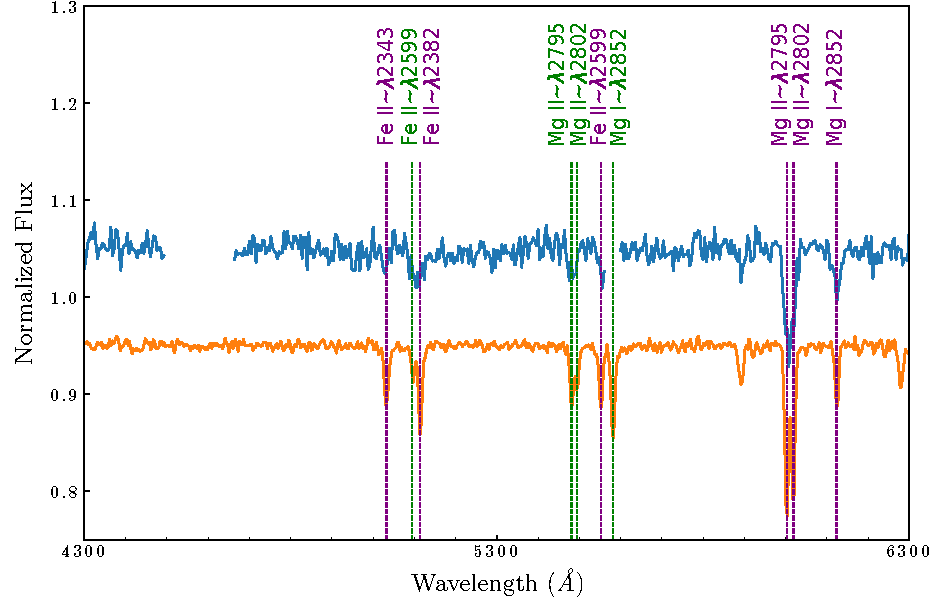
\includegraphics[width = 1.0\textwidth]{4_grb191221_abs.pdf}
    \caption{Comparison of the normalized (and offset by $\pm 0.05$) spectra as obtained with the \gls{SALT} \gls{RSS} (blue) and the \gls{VLT} \gls{FORS}[2] orange. Note the chip gap and region of sky subtraction from the \gls{RSS} spectrum. Figure adapted from \citep{Buckley191221B}.}
    \label{fig:grb_abs}
\end{figure}

\autoref{fig:grb_abs} shows the normalized spectra of the \gls{SALT} \gls{RSS} and \gls{VLT} \gls{FORS}[2] observations, offset by $\pm 0.05$, respectively.
The spectra show a good agreement across the measured position of the proposed absorption features, with the \gls{FORS}[2] spectrum being able to resolve three close pairs of lines, namely, {Fe}\,\textsc{ii} $5096/5114$~\AA, {Mg}\,\textsc{ii} $5481/5494$~\AA, and {Mg}\,\textsc{ii} $6002/6018$~\AA, which were unresolved in the \gls{RSS} spectrum.

\begin{table}[t]

    \centering

    \caption{Properties of the identified absorption lines within the spectra. The measured redshifts of the identified features correspond neatly to two distinct redshifts. Table adapted from \citet{Buckley191221B}.}
    \label{table:grb_lines}

    \begin{tabular}{lccccc}
        \toprule
        Line ID &
        \begin{tabular}[c]{@{}c@{}}Rest\\Wavelength (\AA)\end{tabular} &
        \begin{tabular}[c]{@{}c@{}}Observed\\Wavelength (\AA)\end{tabular} &
        \begin{tabular}[c]{@{}c@{}}\gls{FWHM}\\(\AA)\end{tabular} &
        \begin{tabular}[c]{@{}c@{}}\glsxtrshort{EW}\\(\AA)\end{tabular} &
        $z$ \\
        \midrule
        Fe~II & $2343$ & $5032.35 \pm 1.44$ & $5.44 \pm 1.43$ & $0.83 \pm 0.26$ & $1.148$ \\
        Fe~II & $2599$ & $5096.67 \pm 2.19$ & $4.70 \pm 2.26$ & $0.45 \pm 0.23$ & $0.961$ \\
        Fe~II & $2382$ & $5114.49 \pm 0.90$ & $4.67 \pm 0.96$ & $1.10 \pm 0.23$ & $1.147$ \\
        Mg~II & $2795$ & $5481.56 \pm 1.57$ & $4.10 \pm 1.67$ & $0.67 \pm 0.21$ & $0.961$ \\
        Mg~II & $2802$ & $5494.59 \pm 2.19$ & $3.93 \pm 2.29$ & $0.45 \pm 0.19$ & $0.961$ \\
        Fe~II & $2599$ & $5552.48 \pm 1.25$ & $4.01 \pm 1.25$ & $0.62 \pm 0.19$ & $1.136$ \\
        Mg~I  & $2852$ & $5581.78 \pm 0.91$ & $4.44 \pm 0.91$ & $1.05 \pm 0.22$ & $0.957$ \\
        Mg~II & $2795$ & $6002.98 \pm 0.37$ & $4.56 \pm 0.40$ & $2.08 \pm 0.25$ & $1.148$ \\
        Mg~II & $2802$ & $6018.71 \pm 0.14$ & $4.38 \pm 0.43$ & $1.83 \pm 0.24$ & $1.148$ \\
        Mg~I  & $2852$ & $6124.64 \pm 1.28$ & $4.10 \pm 1.30$ & $0.69 \pm 0.22$ & $1.128$ \\
        \bottomrule
    \end{tabular}

\end{table}


\autoref{table:grb_lines} shows the measured absorption line properties, specifically for the \gls{FORS}[2] spectrum due to its higher \gls{SNR} and better line resolution than the \gls{RSS} spectrum.
Two distinct redshifts were acquired from the absorption line measurements, namely $z = 0.960 \pm 0.0017$ and $z = 1.142 \pm 0.0078$.
Initial analysis of the spectrum by the \gls{Swift}/\gls{UVOT} team \citep{Kuin2019} placed the redshift at $z = 1.19$, which was later further refined by \citet{Vielfaure2019} who reported a redshift for the host galaxy of $z = 1.148$, as well as a fainter intervening system at $z = 0.961$, firmly agreeing with the measured redshifts found with \gls{RSS} and \gls{FORS}[2].

% MARK: HEASA 2021
\subsection[Proceeding, HEASA (2021)]{%
    Development of Tools for the \gls{SALT}/\gls{RSS} Spectro\-polari\-metry Reductions: Application to the Blazar 3C 279\\
    (Proceedings of Science, \glsxtrshort{HEASA} 2021)
}

% Basic background information
As discussed in \citet[][see also \autoref{app:papers}]{Cooper_HEASA2021}, it was shown that alternative wavelength solutions, such as those created using \iraf, are capable of being applied to \gls{SALT} spectro\-polarimetric data.
The `additional tools' mentioned therein, which were the precursor to the \stops\ pipeline, were used during the reduction of the blazar 3C~279.

The blazar 3C~279 was observed in linear spectropolarimetry mode, on $2017$ May $17$, using the PG$0900$ grating with two different grating angles ($12.5$\degree\ and $19.5$\degree).
The grating and articulation angles used for the observations (see \autoref{table:sci_targets}) matched those of observations of the spectrophotometric standard star, Hiltner $600$, observed on $2017$ February $24$, allowing the intensity to be relatively flux calibrated.

\begin{figure}[t]
    \centering
    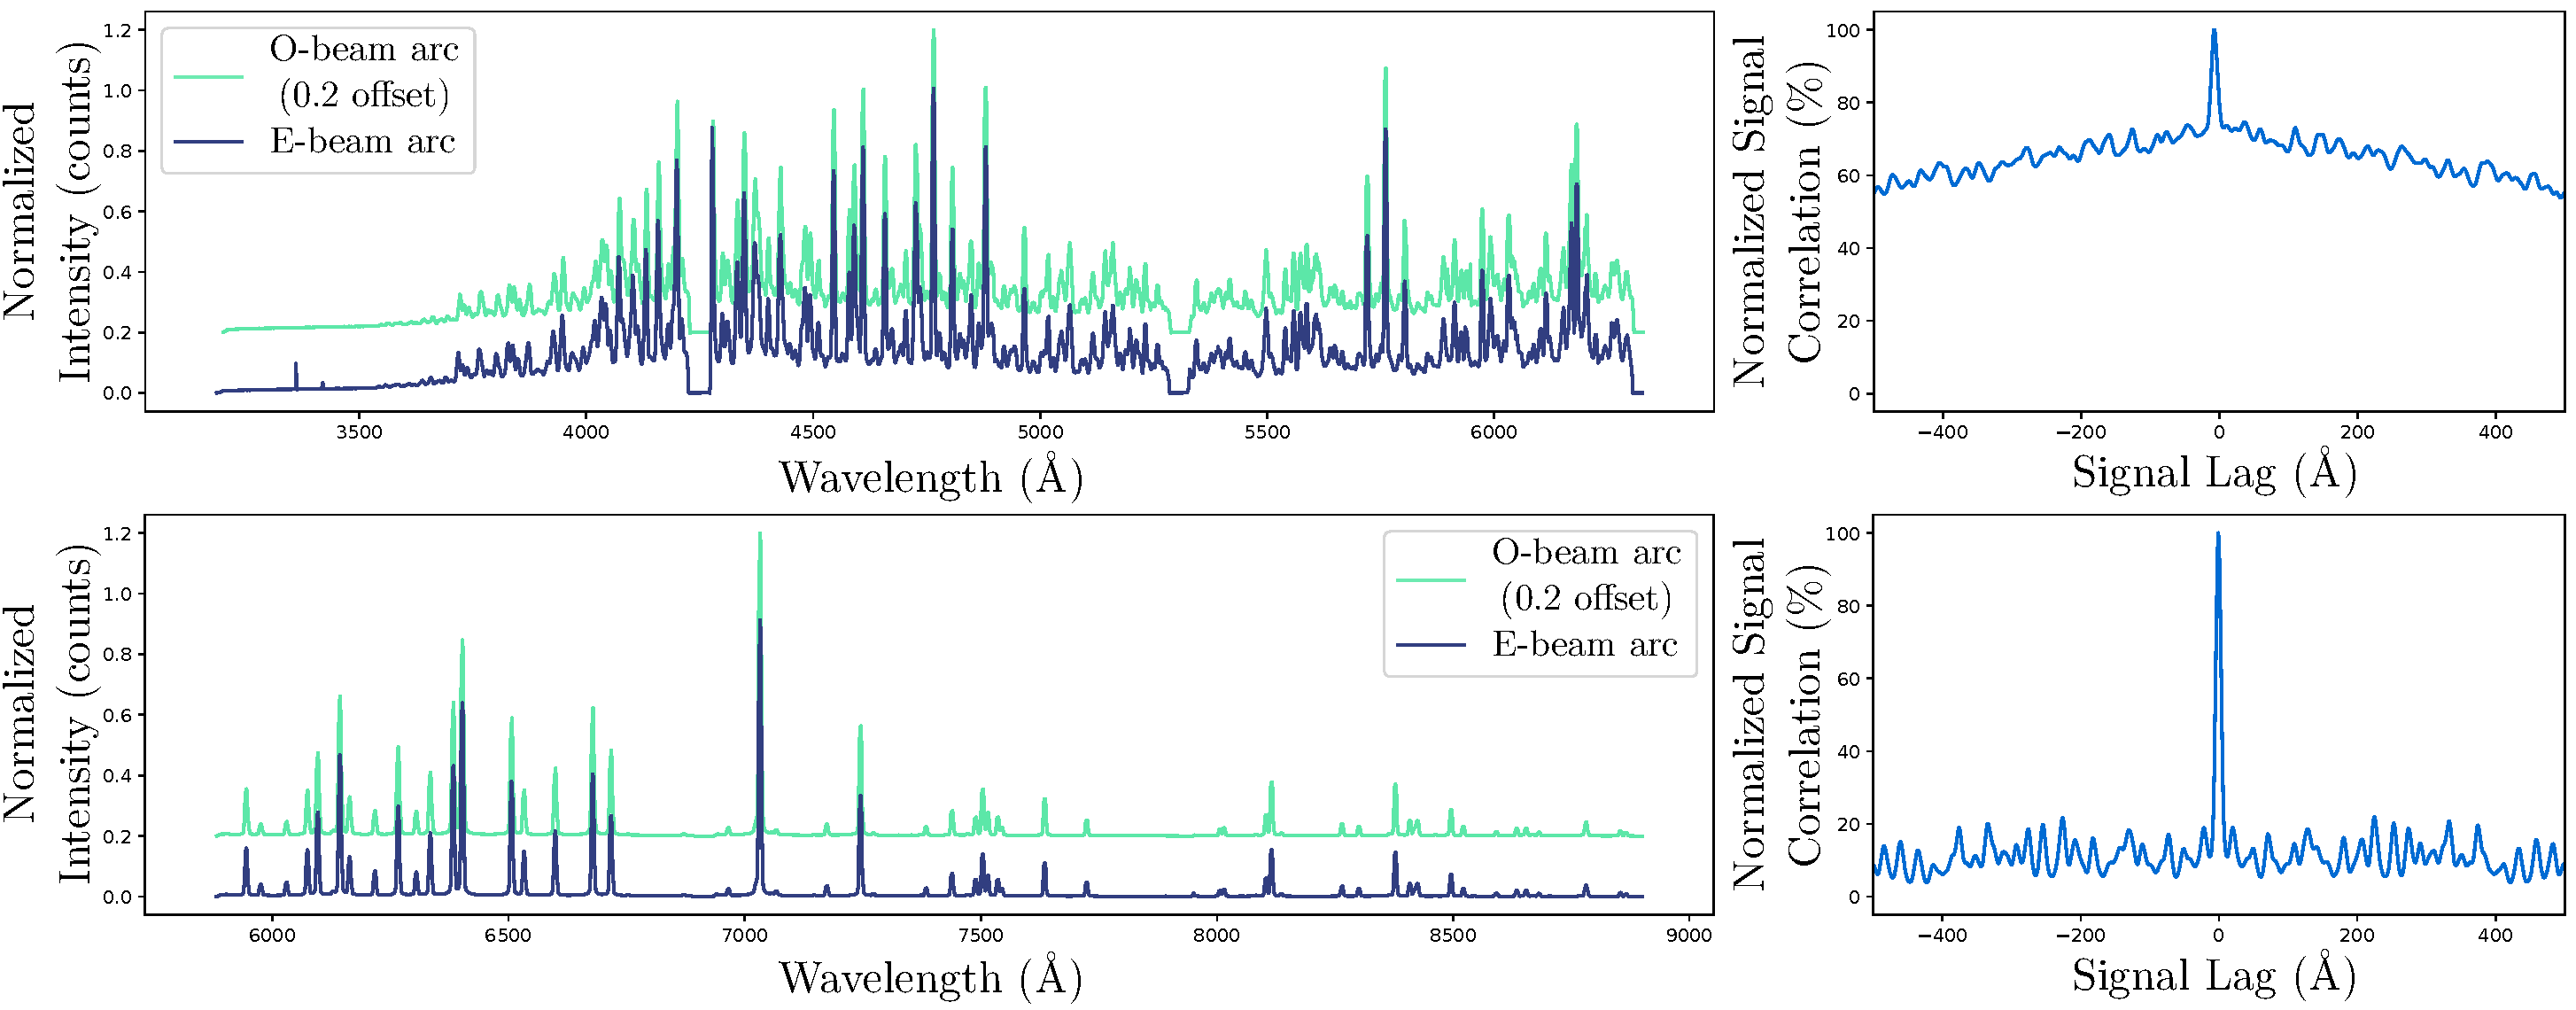
\includegraphics[width = 1.0\textwidth]{4_HEASA2021_oecorr.pdf}
    \caption{The spectra and cross correlation of the $O$- and $E$-beams of the \gls{ThAr} (top) and \gls{NeAr} (bottom) arc lamps. Figure adapted from \citep{Cooper_HEASA2021}.}
    \label{fig:HEASA2021_oecorr}
\end{figure}

\autoref{fig:HEASA2021_oecorr} shows the spectra and cross correlation of the $O$- and $E$-beams of the \gls{ThAr} and \gls{NeAr} arc lamps, also with grating angles of $12.5$\degree\ and $19.5$\degree, respectively.
The cross correlation of the arc lamps perpendicular polarization beams show clear peaks at $0$ lag, indicating that the wavelength solutions are consistent across the two polarization beams.

\begin{figure}[t]
    \centering
    \begin{subfigure}[b]{1.0\textwidth}
        \centering
        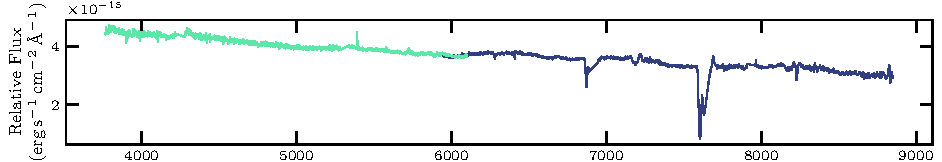
\includegraphics[width = 1.0\textwidth]{4_HEASA_2021_spec.pdf}
        \caption{The relative flux calibration of the 3C~279 spectra.}
        \label{subfig:HEASA2021_spec}
    \end{subfigure}
    \hfill
    \begin{subfigure}[b]{1.0\textwidth}
        \centering
        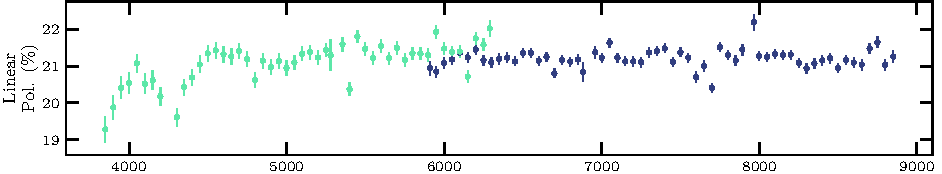
\includegraphics[width = 1.0\textwidth]{4_HEASA_2021_pol.pdf}
        \caption{The linear polarization percentage of the 3C~279 spectra.}
        \label{subfig:HEASA2021_pol}
    \end{subfigure}
    \hfill
    \begin{subfigure}[b]{1.0\textwidth}
        \centering
        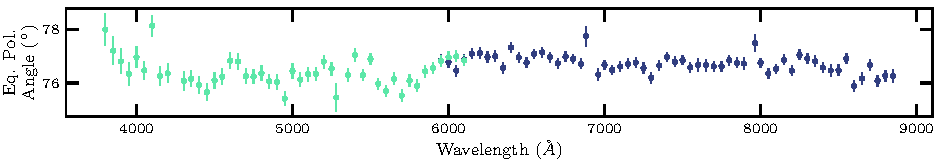
\includegraphics[width = 1.0\textwidth]{4_HEASA_2021_pol_ang.pdf}
        \caption{The polarization angle of the 3C~279 spectra, polarization relative to the instrument.}
        \label{subfig:HEASA2021_pol_ang}
    \end{subfigure}
    \caption{The relative flux calibrated spectra (\subref{subfig:HEASA2021_spec}), linear polarization percentage (\subref{subfig:HEASA2021_pol}), and polarization angle (\subref{subfig:HEASA2021_pol_ang}) of the blazar 3C~279 observed on $2017$ May $17$. Figure adapted from \cite{Cooper_HEASA2021}.}
    \label{fig:HEASA2021}
\end{figure}

\autoref{fig:HEASA2021} shows the relative flux calibrated intensity, percentage of linear polarization, and polarization angle of the blazar 3C~279, across the visible spectrum.
The spectra display a good overlap between the two grating angles, especially when considering the variable nature of blazars as well as the fact that the spectra are only relatively flux calibrated.
Both the percentage of linear polarization and the polarization angle agree well across the grating angle overlap.

% MARK: HEASA 2022
\subsection[Proceeding, HEASA (2022)]{%
    \gls{SALT} Spectropolarimetric Pipeline Comparisons\\
    (Proceedings of Science, \glsxtrshort{HEASA} 2022)
}

As discussed in \citet[][see also \autoref{app:papers}]{Cooper_HEASA2022}, as well as expanding on the work presented in \cite{Cooper_HEASA2021}, it was shown that the \stops\ pipeline has no noticeable effect on the polarization properties of spectropolarimetric data and that the measure of the goodness of fit for the wavelength solutions could be measured, both through correlation and measuring the position of skyline features for both the $O$- and $E$-beams.
The blazar 3C~$279$, the spectrophotometric standard star Hiltner~$600$, and the spectropolarimetric standard star Hiltner~$652$, were observed on the dates tabulated in \autoref{table:sci_targets}.
Observations of 3C~$279$ were taken during periods of enhanced and flaring $\gamma$-ray activity.

\begin{figure}[t]
    \centering
    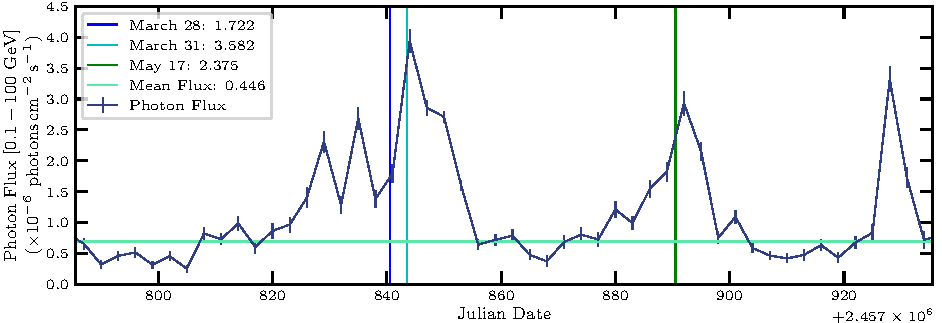
\includegraphics[width = 1.0\textwidth]{4_3C_279_LCR.pdf}
    \caption{The \glsxtrshort{FermiLAT} photon flux [$0.1 - 100$~GeV] for 3C~$279$ as measured around the dates of the \gls{SALT}/\gls{RSS} spectropolarimetric observations (indicated by the vertical lines). Also included are the `mean' $\gamma$-ray fluxes ($\times 10^{-6}$) for the observation dates, calculated using linear interpolation of the \glsxtrshort{FermiLAT} data points. The horizontal turquoise line shows the mean quiescent flux for this source. Figure created using data sourced from the \glsxtrshort{FermiLCR}.\protect\footnotemark}
    \label{fig:3C_279_LCR}
\end{figure}
\footnotetext{\protect\url{https://fermi.gsfc.nasa.gov/ssc/data/access/lat/LightCurveRepository/source.html?source_name=4FGL_J1256.1-0547}}

\autoref{fig:3C_279_LCR} shows the $\gamma$-ray photon flux from 3C~$279$ for energies between $0.1 - 100$~GeV, observed using the \gls{FermiLAT}, as provided by the \glsxtrfull{FermiLCR} \citep{FermiLCR}.
This shows that on the dates of the optical observations, 3C~$279$ was between $\sim4 - 8$ times brighter when compared to its mean quiescent state. 
% was likely at $\gamma$-ray fluxes of $1.72 \times 10^{-6}$, $3.58 \times 10^{-6}$, and $2.38 \times 10^{-6}$~$ph.\,cm^{-2}s^{-1}$, as compared to a quiescent `median' flux of $0.45 \times 10^{-6}$~$ph.\,cm^{-2}s^{-1}$.

\begin{figure}[tp]
    \centering
    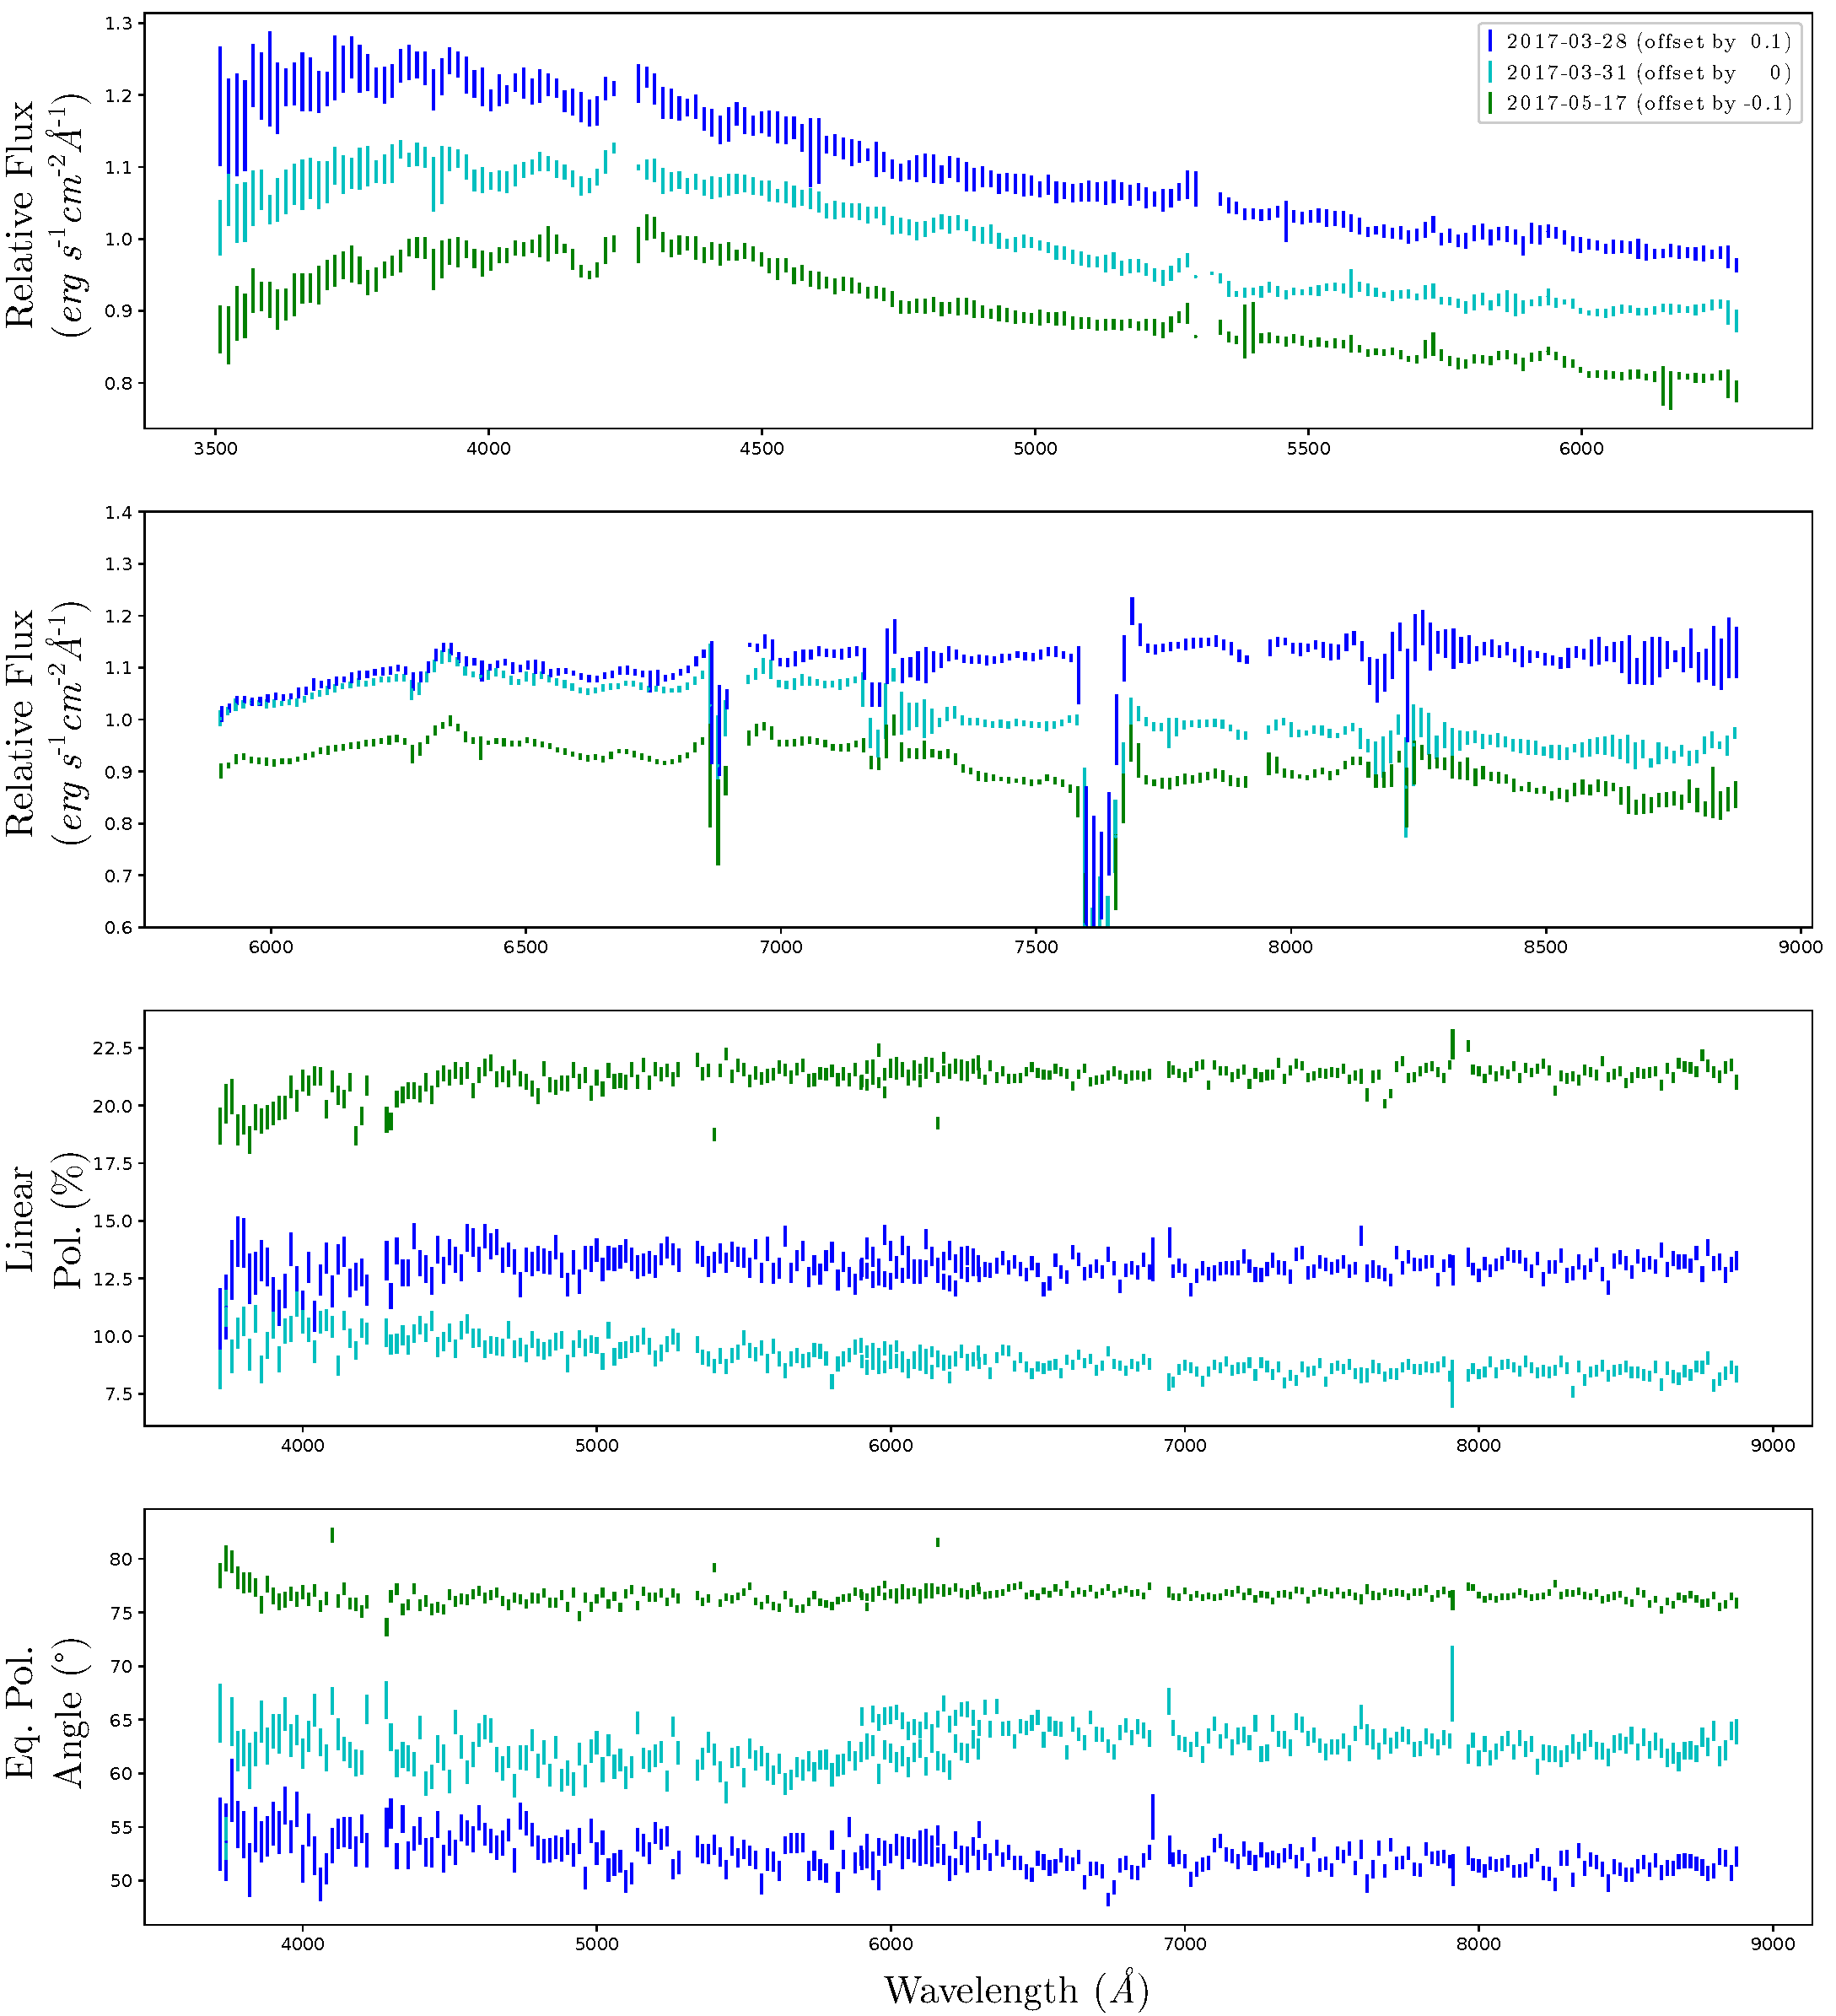
\includegraphics[width = 1.0\textwidth]{4_3C279_all.pdf}
    \caption{Spectropolarimetric results for 3C~$279$ during two distinct periods of flaring. The normalized relative flux is presented for both grating angles, $12.5$\degree (top) and $19.625$\degree (second from top). Figure sourced from \citep{Cooper_HEASA2022}.}
    \label{fig:3C_279_specpol}
\end{figure}

\autoref{fig:3C_279_specpol} shows the spectropolarimetric results for 3C~$279$ during the various states of $\gamma$-ray activity as mentioned above.
The figure shows, from top to bottom, the normalized, relative flux calibrated, spectra for both grating angles ($12.5$\degree\ and $19.625$\degree, observed in that order), the percentage of linear polarization, and the polarization angle.

Although the spectral shape does not vary greatly across the wavelength region, the level of $\gamma$-ray activity during observation has a clear effect on the spectra.
This is most notable for the $2017$ March $31$ observation which displays heightened spectral intensities in the blue.
The linear polarization percentages and polarization angles also show variation over the course of the observations, varying between $\sim 12.23\%$ and $\sim 24.22$\degree, respectively.
There is also good agreement between the polarization properties across the differing grating angles for the same observation dates.
The difference of the polarization percentage and polarization angle between the two grating angles is $\sim 0.25\%$ and $\sim 1.25$\degree, respectively.
The most notable disagreement of the polarization properties is seen, once again, during the $2017$ March $31$ observation, but may be explained due to the flaring state of the blazar, the asynchronous times for the two observations, and a lower \gls{SNR} near the edges of the \gls{RSS}.
% The lower \gls{SNR} could originate from either blaze effects arising from the grating, or from the extraction of the trace, which is currently limited to a rectangular aperture in the current \polsalt\ pipeline.

\begin{figure}[t]
    \centering
    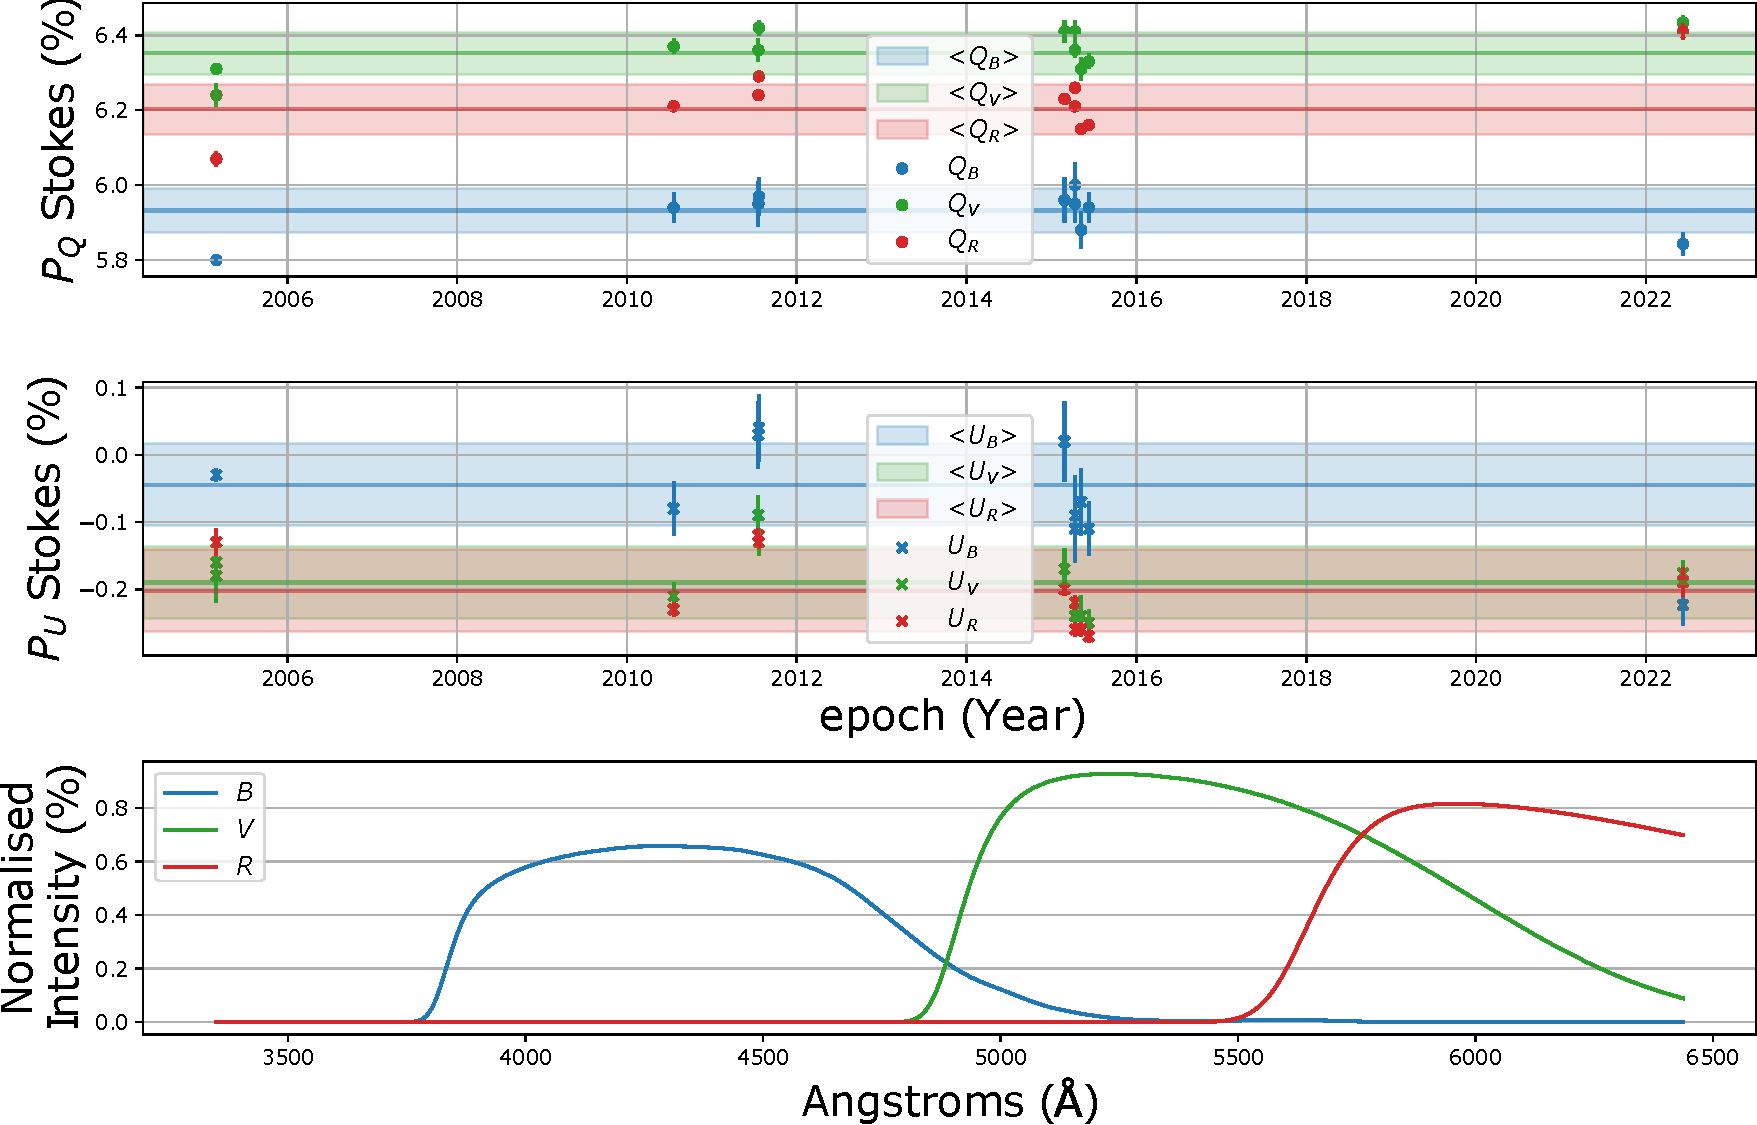
\includegraphics[width = 1.0\textwidth]{4_Hiltner_652.pdf}
    \caption{The reduced $Q$ and $U$ Stokes parameters for Hiltner~$652$, pre$-2006$ for published \glsxtrshort{FORS}[1] data, $2010 - 2016$ for published \glsxtrshort{FORS}[2] data, and post$-2022$ for Stokes parameters observed with \gls{SALT} and convolved with the Johnson-Cousins filter pass-bands. The horizontal lines and shaded regions refer to the \glsxtrshort{FORS} mean and $1\sigma$ regions, respectively. Finally, the bottom plot shows the Johnson-Cousins filter pass-band’s used by \polsalt\ to calculate the Stokes parameters in the different filters. Figure sourced from \citep{Cooper_HEASA2022}.}
    \label{fig:Hilt652}
\end{figure}

\autoref{fig:Hilt652} shows the comparison between the reduced $Q$ and $U$ Stokes parameters for Hiltner~$652$ as observed with the %\glsxtrlong{FORS} (\glsxtrshort{FORS}[1]) and \gls{FORS}[2] mounted at the \gls{VLT} \citep{FORS1, FORS2}, as well as observed with \gls{SALT}.
\glsxtrshort{FORS}[1] and \gls{FORS}[2] \citep[as reported by][]{FORS1, FORS2}, and the \gls{SALT} observations. 
This shows that the Stokes parameters of Hiltner~$652$ are consistent across the different instruments, mostly falling within a standard deviation of historical results.
Minor discrepancies are present, but can be due to multiple compounding effects, such as differing instrumental setups, varying atmospheric conditions, as well as Hiltner~$652$ being classed as a spectrophotometric, and not spectropolarimetric, standard.

% MARK: Schutte - 4C+01.02
\subsection[Schutte et al.\ (2022)]{%
    Modeling the Spectral Energy Distributions and Spectro\-polari\-metry of Blazars - Application to 4C~+01.02 in 2016~$-$ 2017\\
    \citep{Schutte4C0102}
}

\citet{Schutte4C0102} presented the results from spectropolarimetric observations and modeling of the \gls{SED} for the blazar 4C~+$01.02$ during a flaring and a quiescent state.
The optical spectropolarimetric observations of the blazar were completed using the \gls{SALT} \gls{RSS} in spectropolarimetric mode, with observations taken on $2016$ July $09$ and $2017$ July $25$, also noted in \autoref{table:sci_targets}.

\begin{figure}[t]
    \centering
    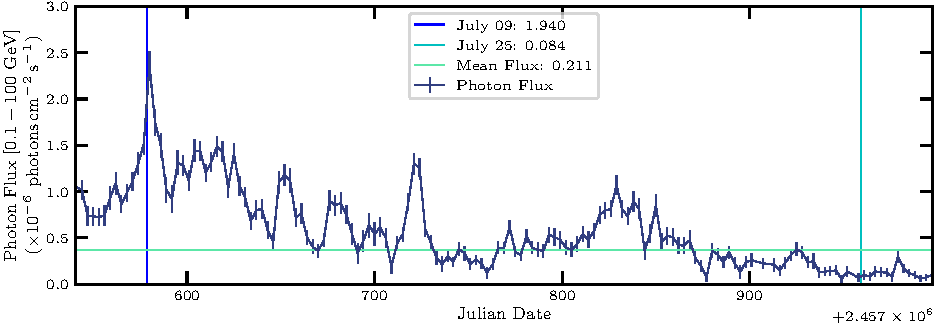
\includegraphics[width = 1.0\textwidth]{4_4C_+01.02_LCR.pdf}
    \caption{The \gls{FermiLAT} photon flux [$0.1 - 100$~GeV] for 4C~+$01.02$ as measured around the dates of the \gls{SALT}/\gls{RSS} spectropolarimetric observations (indicated by the vertical lines). Also included are the `mean' $\gamma$-ray fluxes ($\times 10^{-6}$) for the observation dates, calculated using linear interpolation of the \gls{FermiLAT} data points. The horizontal turquoise line shows the mean quiescent flux for this source. Figure created using data sourced from the \gls{FermiLCR}.\protect\footnotemark}
    \label{fig:4C_+01.02_LCR}
\end{figure}
\footnotetext{\protect\url{https://fermi.gsfc.nasa.gov/ssc/data/access/lat/LightCurveRepository/source.html?source_name=4FGL_J0108.6+0134}}

\autoref{fig:4C_+01.02_LCR} shows the photon flux of 4C~+$01.02$ for $0.1 - 100$~GeV energies as provided by the \gls{FermiLCR}.
The figure shows that during the optical observations of 4C~+$01.02$, the source was at $\gamma$-ray fluxes of $F \approx 1.9 \times 10^{-6}$ and $F \approx 0.1 \times 10^{-6}$~ph.\,cm$^{-2}$\,s$^{-1}$, as compared to a quiescent `median' flux of $\left\langle F \right\rangle = 0.21 \times 10^{-6}$\,ph.\,cm$^{-2}$\,s$^{-1}$.

\begin{figure}[t]
    \centering
    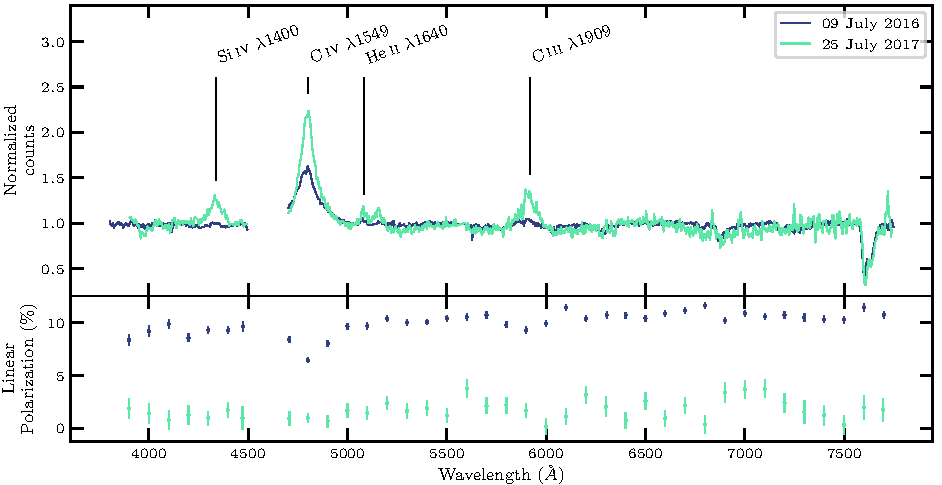
\includegraphics[width = 1.0\textwidth]{4_4C_+01.02_spec.pdf}
    \caption{Spectropolarimetric results for 4C~+$01.02$ during periods of flaring and quiescence. The spectra presented have been continuum subtracted and normalized. Figure adapted from \citep{Schutte4C0102}.}
    \label{fig:4C_01.02_specpol}
\end{figure}

% \autoref{fig:4C_01.02_specpol} shows the spectropolarimetric results for 4C~+$01.02$ during the periods of flaring and quiescence in $2016$ and $2017$, respectively.
% The figure shows 

The normalized, continuum-subtracted, intensity spectra as well as the polarization percentage for the $2016$ and $2017$ epochs are presented in \autoref{fig:4C_01.02_specpol}.
The spectral features were identified using the known redshift of 4C~$01.02$ of $z = 2.1$.
The quiescent state spectrum exhibits more prominent features than during the flaring state, with the C\,\textsc{iv} line being the most prominent feature present in both spectra.
The increase in the spectral line intensity during the quiescent $\gamma$-ray state is due to the non-thermal continuum emission being fainter, as compared to the flaring state.
% , which dominates the spectrum during the flaring state.

The linear polarization percentages averaged $10.04 \pm 1.03\%$ and $1.72 \pm 0.93\%$ during flaring and quiescence, respectively.
% , which agrees with the prediction that blazars release highly polarized synchrotron emission during periods of flaring.

\pagebreak

The \stops\ pipeline has already proven its worth, aiding in the reduction of numerous spectropolarimetric observations beyond the select few presented above \citep[see e.g.,][]{Barnard_2024}.
Wavelength calibrations are, by far, the most time consuming part of spectropolarimteric data reductions.
The \stops\ software enables faster and thorough wavelength calibrations through external tools, such as \iraf, as well as providing methods to ensure the accuracy of the produced wavelength solutions.
This decreases the time necessary for reductions while still ensuring their accuracy, allowing the analysis of the results to take precedence.
